\section{Experiments on synthetic datasets}
In this section we report some numerical experiments to highlight the effects of the proposed techniques on the training process. In all the experiments with artificial dataset we employed a potentially infinite training-set, since we generate data on the fly. We used a validation set to determine the success of the training process. We define a training run to be successful if the error on the validation set if less than 1\%. The error is clearly defined for each task, see Appendix \ref{app:tasks} for more details on the tasks. We say a run as unsuccessful is the loss do not decrease for more than $3\cdot 10^6$ iterations. The validation test is composed by $10^4$ examples of different lengths sampled once at the beginning. In all the experiments we used RNNs with 50 hidden units trained with a learning rate of $10^{-3}$, clipping threshold of $1$, batch size equal to $100$, initial spectral radius of $1.2$. We did not experiment much on the batch size. We found instead that the this combination of learning rate and threshold is generally good for all the task and lengths, although for tasks with smaller sequences more aggressive learning rate can be used.

\subsection{The effect of the spectral initialization}

For this experiment we consider the temporal order task which has always been considered effectively impossible to solve using a plain version of the stochastic  gradient descent algorithm.
In \cite{advancesInOptimizingRnns}, for instance, are reported the rate of success of SGD and SGD modified with gradient clipping technique for such a task with different input lengths. It shows that for sequences longer than 20 neither one of the algorithms can solve the problem. We repeated the same experiment, namely training the network varying the length\footnote{Here we refer as the length of the task to the minim length of the input sequences} of the input sequences, with the SGD algorithm modified with the gradient clipping technique (SGD-C) using our initialization scheme. 
%In figure \ref{fig:spectral_init_effect} are shown the number of iterations (means of 5 different runs with different random seeds) required to solve the problem for lengths in [50 100 150 200]. The important thing to notice is that, contrarily to what commonly believed, it is possible to train RNNs with SGD (with gradient clipping): not one of the runs for any length failed.

In Figure \ref{fig:temporal_rates} we compare the rate of success between an initialization scheme using only a standard Gaussian initialization, and the initialization scheme by us proposed where $\mat{W}_{rec}$ is scaled to have spectral radius larger than one. We notice that scaling the recurrent matrix has a huge effect on the rate of success: where the standard scheme failed for sequences longer than 20, with the spectral initialization we managed to succeed up to sequences of length 150.

\begin{figure}
	\centering
	\includegraphics[width= 0.9\textwidth]{chapter4/temporal_rates.png}
	\caption{Rate of success (mean of 5 runs) for the temporal order task for various lengths with SGD modified with gradient clipping. In blue and red the results when $W_{rec}$ is initialized with spectral radius bigger and smaller than one respectively.}
	\label{fig:temporal_rates}
\end{figure}

%\begin{figure}
%	\centering
%	\includegraphics[width= 0.9\textwidth]{chapter4/spectral_init_exp.eps}
%	\caption{Number of iterations (means of 5 different random seed) needed to solve the task for different lengths}
%	\label{fig:spectral_init_effect}
%\end{figure}


\subsection{The effect of using the simplex direction}
The first experiment we ran is developed to compare the simplex strategy and the variant with the conditional switching to the anti-gradient with the standard SGD. We tested the three algorithms on the addition problem (T=100). In Figure \ref{fig:comparisong_add_simplex} is shown the loss on the validation set during the training process (until convergence). 

The first part of the learning process is particularly interesting because it highlights the differences between the simplex and the anti-gradient direction in the regime of vanishing gradients. In the anti-gradient case the loss remains roughly constant for a good portion of the whole training time until it starts decreasing significantly. The other two strategies perform differently. In fact they both start decreasing a lot sooner in all the three runs. This should suggests that using the simplex direction helps the training process when the gradient is vanishing, which happens in the first part of the training. 

In the second part of the training process, i.e., when the loss is decreasing, relatively rapidly, gradients do not vanish and moreover have large norm. We can see from the plots that the simplex direction can perform poorly in this second part compared to the anti-gradient one. So, the idea of switching back to the ant-gradient direction in this phase proves to be beneficial.

%\begin{figure}
%	\centering
%	\includegraphics[width= 0.8\textwidth]{chapter4/compare_add_simplex.png}
%	\caption{Comparison between SGD using as descent direction the anti-gradient (in yellow, converges for last), the simplex direction (in purple, converges for second) and the simplex direction with conditional switching (in red, converges for first) for the addition task (T=100). In y axis the loss (mean squared error) in logarithmic scale.}
%	\label{fig:comparisong_add_simplex}
%\end{figure}


\begin{figure}
	\begin{subfigure}{1.\textwidth}
		\centering
		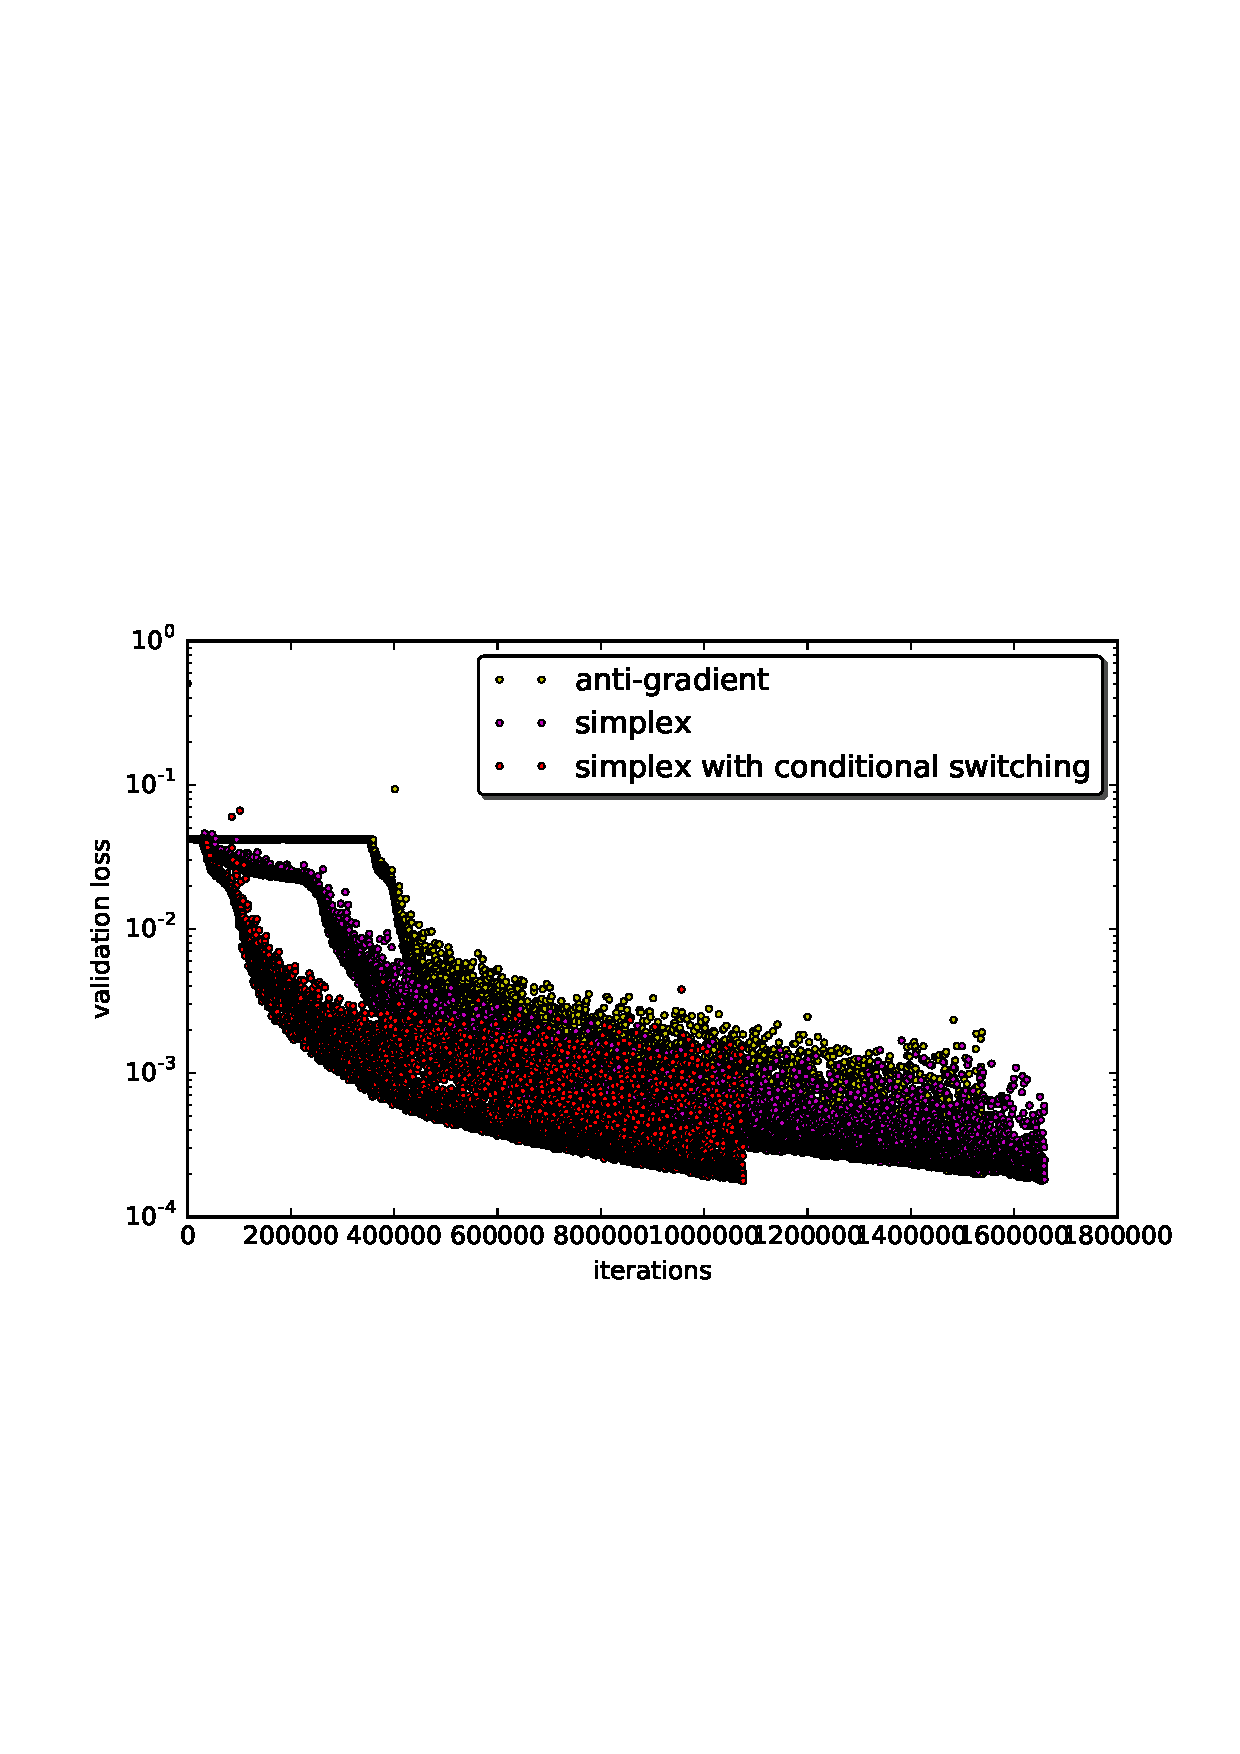
\includegraphics[width= 1\textwidth]{chapter4/compare_add_simplex_13.png}
		\caption{First run}
		\label{fig:a:comparisong_add_simplex}
	\end{subfigure}\\
	\begin{subfigure}{1.\textwidth}
		\centering
		\includegraphics[width= 1\textwidth]{chapter4/compare_add_simplex_14.png}
		\caption{Second run}
		\label{fig:b:comparisong_add_simplex}
	\end{subfigure}\\
	\begin{subfigure}{1.\textwidth}
		\centering
		\includegraphics[width= 1\textwidth]{chapter4/compare_add_simplex_15.png}
		\caption{Third run}
		\label{fig:c:comparisong_add_simplex}
	\end{subfigure}%
	\caption{Comparison between SGD using as descent direction the anti-gradient (in yellow, start decreasing always for last), the simplex direction (in purple, which is the second that start decreasing) and the simplex direction with conditional switching (in red, start decreasing always for first) for the addition task (T=100). In y axis the loss (mean squared error) in logarithmic scale.}
	\label{fig:comparisong_add_simplex}
\end{figure}

In Table \ref{table:add_100_comparison_iterations} are shown the number of iterations (mean values of 3 runs) needed for convergence for each strategy. Notice that the simplex direction with conditional switching obtains the best result.
\begin{table}
	\centering
	\begin{tabular}{C{2cm} | C{2cm} | C{4cm}}
		anti-gradient & simplex & simplex with conditional switching \\
		1807466 & 2338500 & 1630666 \\
	\end{tabular}
	\caption{Number of iterations until convergence for the addition task (T=100). Mean of 3 runs.}
	\label{table:add_100_comparison_iterations}
\end{table}

We repeated the experiment also for the temporal order task (T=100) and we found that also in this case the simplex direction with conditional switching outperforms the anti-gradient. In particular the anti-gradient strategy succeeded in only two out of three runs while the simplex with conditional switching managed to succeed in all the three runs. Furthermore such strategy is sensibly faster than the anti-gradient one. In Table \ref{table:torder_100_comparison_iterations} is shown the mean, computed only on the successful runs, number of iterations needed for convergence for the anti-gradient and the simplex with conditional switching strategies.

\begin{table}
	\centering
	\begin{tabular}{C{2cm} | C{4cm}}
		anti-gradient & simplex with conditional switching \\
		2164800 & 1010000 \\
	\end{tabular}
	\caption{Number of iterations until convergence for the temporal order task (T=100). The mean is computed only on the successful runs: 2/3 for the anti-gradient and 3/3 for the simplex with conditional switching.}
	\label{table:torder_100_comparison_iterations}
\end{table}
